
% \subsection{Experience}
% \ShowTOC

\newcommand{\HighlightRow}{\rowcolor{structure.fg!30}}

\begin{frame}{Application Experience}%{A Sub-title is optional}
\begin{itemize}
\item Jetty webserver
  \begin{itemize}
  \item 11 versions, 5.1.0 through 5.1.10, 1.5 years
  \item 45 KLOC
  \end{itemize}
\item JavaEmailServer
  \begin{itemize}
  \item 10 versions, 1.2.1 through 1.4, 2 years
  \item 4 KLOC
  \end{itemize}
\item CrossFTP server
  \begin{itemize}
  \item 4 versions, 1.05 through 1.08, more than a year
  \item 18 KLOC
  \end{itemize}
\end{itemize}
\end{frame}

\begin{frame}{What works}%{A Sub-title is optional}
\begin{center}
{\Large Support 20 of 22 updates}
\end{center}
\vspace{2ex}
\begin{itemize}
\item 13 updates change class signature by adding new fields
\item Several updates require On-stack replacement support
\item Two versions update an infinite loop, postponing the update
indefinitely
\end{itemize}
\end{frame}

% \begin{frame}{Unsupported updates}%{A Sub-title is optional}
% \begin{itemize}
% \item JavaEmailServer 1.2.4 to 1.3
%   \begin{itemize}
%   \item Update reworks the configuration framework of the server
%   \item Many classes are modified to refer to the configuration system
%   \item Including infinite loops in SMTP and POP threads
%   \end{itemize}
% \item Jetty 5.1.2 to 5.1.3
%   \begin{itemize}
%   \item The application would never reach a safe point
%   \item Modified method {\tt ThreadedServer.acceptSocket()} that waits for
%         connections is nearly always on stack
%   \item Return barrier not sufficient since the main method in other
%         threads {\tt PoolThread.run()} is itself modified
%   \end{itemize}
% \end{itemize}
% \end{frame}

\begin{frame}{\DSU{} performance}%{A Sub-title is optional}
\begin{center}
{\Large No overhead during steady-state execution}
\end{center}
\vspace{1ex}
\begin{center}
\scalebox{0.9}{\includegraphics{graphs/only-jvolve-throughput-latency}}%
\end{center}
% \begin{itemize}
% \item No apriori overhead during normal execution \\
% (before and after the update)
% \item Only effect on execution time is the update pause time
%   \begin{itemize}
%   \item Comparable to GC pause time
%   \end{itemize}
% \end{itemize}
% \begin{large}
% \begin{eqnarray*}
% \text{DSU Pause Time} & \approxeq & \text{Regular GC Time} + \\ 
%                       &           & \text{Time to allocate upd. objects} + \\
%                       &           & \text{Time to transform objects} \\
%                       & \propto   & \text{Upd. objects fraction} \\
%                       &           & \text{Heap size}
% \end{eqnarray*}
% \end{large}
\end{frame}

% \begin{frame}{Jetty webserver performance}%{A Sub-title is optional}
% \begin{itemize}
% \item Used \texttt{httperf} to issue requests
% \item Both client and server on a the same machine, \\
% an Intel Core 2 Quad
% \item Report throughput and latency, median of 21 runs
% % \item Create 800 new connections/second (saturation rate)
% % \item 5 serial requests to 40KB file per connection
% % \item Compared versions 5.1.5 and 5.1.6
% % \item Experiments on Intel Core 2 Quad, Linux 2.6.22, JikesRVM SVN r15532
% \end{itemize}
% \end{frame}
% 
% \begin{frame}{Jetty webserver: Throughput and latency measurements}%{A Sub-title is optional}
% \begin{center}%
% \scalebox{0.9}{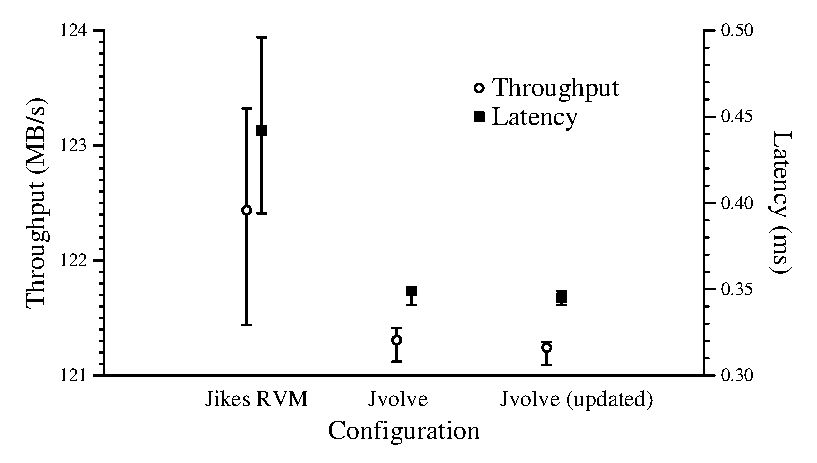
\includegraphics{graphs/jetty-throughput-latency}}%
% \end{center}%
% \end{frame}

% \begin{frame}{DSU pause times}%{A Sub-title is optional}
% \begin{itemize}
% \item \DSU{} performs a GC to transform objects
% \item Pause time determined by
%   \begin{itemize}
%   \item Heap size
%   \item \# of objects transformed
%   \end{itemize}
% \item Simple microbenchmark varying the fraction of objects transformed in
% a 1GB heap
% \end{itemize}
% \end{frame}

% \begin{frame}{DSU pause times (microbenchmark)}%{A Sub-title is optional}
% \begin{center}%
% 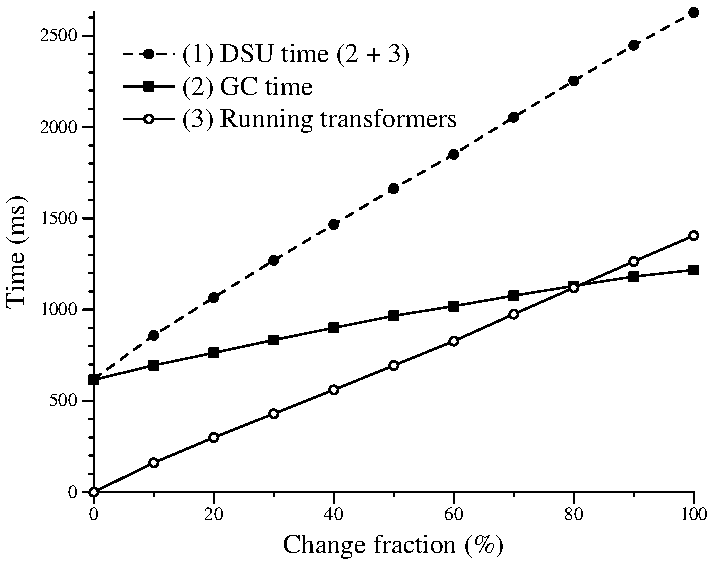
\includegraphics[scale=.8]{graphs/microbench}%
% \end{center}%
% \end{frame}

% \begin{frame}{Jetty webserver: Summary of changes}%{A Sub-title is optional}
% \begin{footnotesize}
% \begin{center}
% \begin{tabular}{|l||c||c|c|c|r|c|c|} \hline
% Ver.    & \#      & \multicolumn{6}{c|}{\# changed} \\
%         & classes & classes & \multicolumn{3}{c|}{methods} & \multicolumn{2}{c|}{fields} \\
%         & added   &         & add & del & chg              & add & del \\ \hline \hline
% 5.1.1   & 0       & 14      & 4   & 1   & 38/0             & 0   & 0   \\
% 5.1.2   & 1       & 5       & 0   & 0   & 12/1             & 0   & 0   \\ \HighlightRow
% 5.1.3   & 3       & 15      & 19  & 2   & 59/0             & 10  & 1   \\ \HighlightRow
% 5.1.4   & 0       & 6       & 0   & 4   & 9/6              & 0   & 2   \\ \HighlightRow
% 5.1.5   & 0       & 54      & 21  & 4   & 112/8            & 5   & 0   \\ \HighlightRow
% 5.1.6   & 0       & 4       & 0   & 0   & 20/0             & 5   & 6   \\ \HighlightRow
% 5.1.7   & 0       & 7       & 8   & 0   & 11/2             & 9   & 3   \\
% 5.1.8   & 0       & 1       & 0   & 0   & 1/0              & 0   & 0   \\
% 5.1.9   & 0       & 1       & 0   & 0   & 1/0              & 0   & 0   \\
% 5.1.10  & 0       & 4       & 0   & 0   & 4/0              & 0   & 0   \\ \hline
% \end{tabular}
% \end{center}
% \end{footnotesize}
% \end{frame}

